\documentclass{article}
\usepackage{spconf,amsmath,graphicx,booktabs,array,url}
\usepackage[T1]{fontenc}

\graphicspath{{figures/}}
\urlstyle{same}

\name{Hequn Lan}
\address{School of Information Engineering\\Guangdong University of Technology\\Guangzhou, China}
\title{Hardware-Calibrated Progressive Temporal Reuse for Efficient Video Semantic Segmentation}

\begin{document}
\ninept
\maketitle

\begin{abstract}
Temporal reuse can reduce redundant video segmentation work, but a fixed reuse policy does not account for frame-wise drift or target-device stage costs. We present Hardware-Calibrated Progressive Reuse (HCPR), a lightweight controller for SegFormer that chooses among whole-stage continuation routes from measured temporal drift, normalized drift scales, and target-device marginal stage costs. HCPR keeps the model, decoder, precision, and data protocol fixed; it changes only which cached stage suffix is reused on each frame. On the VSPW validation split, HCPR transfers from an RTX 4090 D to an RTX 3080 Ti without retraining or lambda recalibration. At its lowest-damage tested point, it obtains 1.354$\times$ speedup with 0.0726 mIoU points of loss for B0 and 1.344$\times$ with 0.1193 points for B1. These results support scoped cross-device robustness, while also showing that target-device stage-cost profiling remains necessary.
\end{abstract}

\begin{keywords}
video semantic segmentation, temporal feature reuse, hardware-aware inference, SegFormer, VSPW
\end{keywords}

\section{Introduction}
Video semantic segmentation repeatedly applies an image model to frames that often contain substantial temporal redundancy. Keyframe propagation and multi-rate execution exploit this redundancy \cite{zhu2017dff,shelhamer2016clockwork,jain2019accel}, but a practical controller must answer two coupled questions: how much of a hierarchical model can be reused on the current frame, and which reuse decision is worthwhile on the target GPU? A fixed interval or fixed boundary cannot express both temporal drift and unequal stage costs.

Our starting point is the controlled whole-stage reuse study from the preceding round. It established a measurable quality--latency trade-off for reusing SegFormer suffixes, but it used fixed routes and did not adapt their allocation per frame. We therefore study a deliberately narrow extension: progressive whole-stage decisions inside the frozen SegFormer-B0/B1 pipeline. The decoder and the fresh prefix remain active, and no token sparsity, architectural change, or low-level kernel is introduced.

We make three contributions:
\begin{itemize}
\item We formulate HCPR as a progressive controller over the whole-stage actions $\{\mathrm{S2\mbox{-}S4},\mathrm{S3\mbox{-}S4},\mathrm{S4},\mathrm{Full}\}$, using per-boundary temporal drift and an explicit age guard.
\item We normalize the controller with lightweight target-device stage-cost measurements, transferring frozen temporal scales and thresholds without retraining or validation-mIoU tuning.
\item We evaluate the same HCPR semantics on VSPW with SegFormer-B0/B1 and RTX 4090 D/RTX 3080 Ti, including paired end-to-end latency, physical stage-call counters, and cross-device ablations.
\end{itemize}

\section{Related Work}
\textbf{Temporal feature reuse.} Deep Feature Flow propagates features from keyframes \cite{zhu2017dff}, while Clockwork Convnets assign different execution rates to network components \cite{shelhamer2016clockwork}. Accel combines efficient segmentation with corrective fusion \cite{jain2019accel}. These studies motivate exploiting temporal redundancy, whereas HCPR focuses on auditable whole-stage choices in a hierarchical Transformer.

\textbf{Efficient video segmentation.} Video methods have explored temporally consistent propagation \cite{baghbaderani2024bofp}, dynamic token processing \cite{liu2024dovit}, resolution changes for compressed video \cite{hu2023arseg}, and temporal adaptation \cite{zhang2022auxadapt}. Temporal Feature Correlation (TFC) further studies selective reuse with alignment and correction \cite{lin2024tfc}. HCPR is intentionally narrower: it adds no alignment, fusion, or learned selector to the frozen segmentation model.

\textbf{Segmentation Transformers.} SegFormer uses a hierarchical Mix Transformer encoder and a lightweight multi-scale decoder \cite{xie2021segformer}; VSPW supplies the video scene parsing benchmark used here \cite{miao2021vspw}. RTFormer represents a complementary approach that designs a real-time Transformer segmentation model directly \cite{wang2022rtformer}. Our question is orthogonal to architecture design: whether measured stage economics can guide reuse across two devices.

\section{HCPR}
\subsection{Progressive whole-stage contract}
Let $F_i(t)$ denote the output of stage $i$ for frame $t$. The frozen SegFormer path is
\begin{equation}
 F_1(t) \rightarrow F_2(t) \rightarrow F_3(t) \rightarrow F_4(t) \rightarrow D(t),
\end{equation}
where $D$ is the decoder. HCPR always computes $F_1$ and $D$. On a non-full frame it selects one continuation route:
\begin{equation}
\begin{aligned}
 \mathrm{S2\mbox{-}S4}:&\quad D(F_1(t),\widehat F_2,\widehat F_3,\widehat F_4),\\
 \mathrm{S3\mbox{-}S4}:&\quad D(F_1(t),F_2(t),\widehat F_3,\widehat F_4),\\
 \mathrm{S4}:&\quad D(F_1(t),F_2(t),F_3(t),\widehat F_4).
\end{aligned}
\end{equation}
Here a hat is a cached final stage output, not an estimate of the current feature. A Full action computes and updates all stages. Cache state resets at each video boundary; the first frame is Full. A stopped suffix is absent from the forward path rather than computed and masked.

\begin{figure}[t]
  \centering
  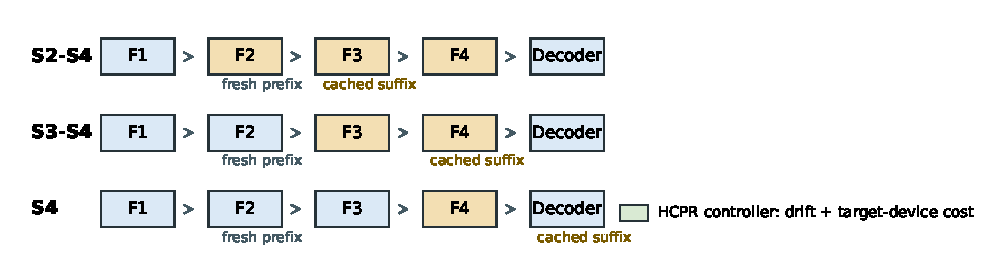
\includegraphics[width=\columnwidth]{hcpr_method.pdf}
  \caption{HCPR selects a progressive whole-stage route. The fresh prefix and cached suffix change by action, while the decoder remains active on every frame.}
  \label{fig:method}
\end{figure}

\subsection{Drift and hardware-calibrated score}
HCPR stores the final outputs $C_2,C_3,C_4$ from the latest refresh. It also stores the pooled references $R_{1\to2}$, $R_{2\to3}$, and $R_{3\to4}$. For progressive boundary $i\in\{1,2,3\}$, the FP32 drift is
\begin{equation}
 d_i(t)=1-\cos\!\left(\operatorname{GAP}(F_i(t)),R_{i\to i+1}\right),\qquad z_i(t)=\frac{d_i(t)}{s_i+\epsilon}.
\end{equation}
The scale $s_i$ is the p90 drift scale estimated from 32 training videos with labels unused. Let $c_i$ be the target-device marginal cost of stage $i$ and $T_{\mathrm{full}}$ the measured full profile. We use
\begin{equation}
 k_i=\frac{c_i}{T_{\mathrm{full}}},\qquad q_i(t)=\frac{z_i(t)}{k_{i+1}},
\end{equation}
to compare the next continuation with its target-device cost. HCPR proceeds through a boundary when $q_i(t)>\lambda$; otherwise it stops and reuses the remaining suffix. The score thresholds are frozen quantiles $20,35,50,65,80,90,95$ from the Round 11A calibration. An age guard forces a Full refresh after at most seven consecutive stale frames.

Only $c_2,c_3,c_4$ and $T_{\mathrm{full}}$ are remeasured on the target GPU. The drift scales, lambdas, weights, precision, resolution, decoder, and cache semantics remain frozen. Thus the supported deployment statement is that target-device stage-cost profiling is required, while lambda recalibration is not required for the evaluated transfer.

\section{Experimental Protocol}
\textbf{Data and models.} We use the official VSPW validation split: 343 videos, 24,392 RGB/ground-truth pairs, 124 classes, and ignore label 255 \cite{miao2021vspw}. We evaluate frozen VSPW-compatible SegFormer-B0 and B1 checkpoints. The input is $512\times512$, batch size is one, and compute uses BF16 autocast. No model, split, resolution, decoder, or training procedure changes between devices.

\textbf{Calibration and timing.} HCPR is calibrated on 32 training videos with seed 42 and labels unused. Lambda values are score quantiles and are not selected by validation mIoU. Both devices use CUDA 11.8, PyTorch 2.1.2+cu118, and Transformers 4.44.2; the driver versions differ, so this is cross-device validation under matched framework/runtime versions. The timing boundary is a CUDA-resident model input tensor through ready segmentation logits. It includes the fresh prefix, HCPR controller, selected suffix, and decoder, but excludes video decoding, disk I/O, pageable host-to-device transfer, visualization, and file writing. Each configuration uses 200 warmup iterations, 1,000 CUDA-event measurements, five repetitions, and an immediately paired Full baseline in the same process.

\section{Results}
\subsection{Cross-device quality--latency results}
Table~\ref{tab:cross} reports the three anchor quantiles from the frozen HCPR-NewCost route. Each cell is paired speedup / mIoU damage in percentage points. The 4090 D values are Round 11A results; the 3080 Ti values are the independent Round 11B transfer.

\begin{table*}[t]
\centering
\caption{HCPR-NewCost cross-device results. Speedup is measured end-to-end against an immediately paired Full baseline; damage is mIoU points.}
\label{tab:cross}
\scriptsize
\setlength{\tabcolsep}{5pt}
\begin{tabular}{llccc}
\toprule
Model & Device & q20 & q65 & q95 \\
\midrule
B0 & RTX 4090 D & 1.229 / 0.073 & 1.657 / 0.442 & 1.836 / 1.379 \\
B0 & RTX 3080 Ti & \textbf{1.354 / 0.073} & \textbf{1.838 / 0.428} & 2.010 / 1.394 \\
B1 & RTX 4090 D & 1.323 / 0.115 & 1.707 / 0.830 & 1.919 / 2.122 \\
B1 & RTX 3080 Ti & \textbf{1.344 / 0.119} & 1.849 / 0.875 & \textbf{2.093 / 2.179} \\
\bottomrule
\end{tabular}
\end{table*}

The lowest-damage tested points on the second GPU are B0 q20 at 1.354$\times$ with 0.0726 points of loss and B1 q20 at 1.344$\times$ with 0.1193 points. The fastest primary point is B1 q95 at 2.093$\times$, with 2.179 points of loss. The qualitative ordering transfers: a more permissive threshold exposes higher speed, while damage grows. The result is cross-device robustness for the two evaluated scales and GPUs, not a claim of universal GPU portability.

\begin{figure*}[t]
  \centering
  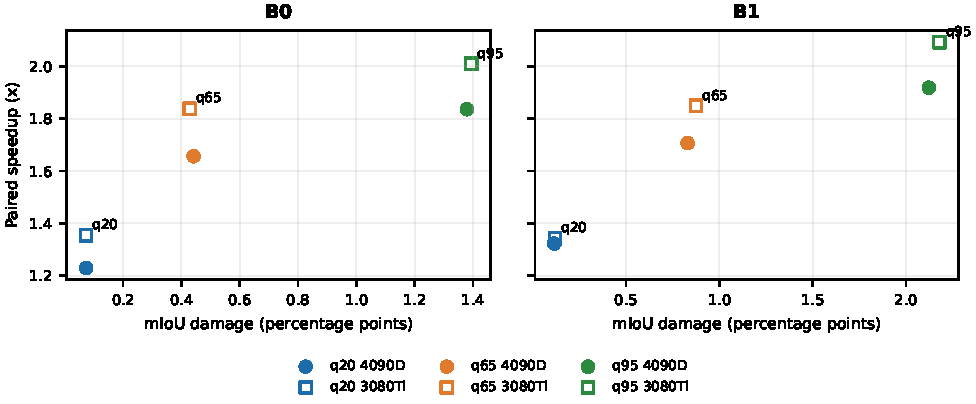
\includegraphics[width=0.72\textwidth]{hcpr_cross_hardware_pareto.pdf}
  \caption{Matched HCPR-NewCost anchor points on the two evaluated GPUs. Filled circles are RTX 4090 D; open squares are RTX 3080 Ti. Values use the same frozen model and temporal calibration.}
  \label{fig:cross}
\end{figure*}

\subsection{Physical computation and controller cost}
The cross-device transfer changes only the stage-cost vector. Table~\ref{tab:profile} lists the measured vectors for both models and devices. Table~\ref{tab:calls} gives the physical q20 counters. Stage 1 and the decoder remain full-rate while stopped suffix work is absent; the maximum stale run is seven for all tested variants.

\begin{table}[t]
\centering
\caption{Physical q20 stage calls on RTX 3080 Ti.}
\label{tab:calls}
\scriptsize
\setlength{\tabcolsep}{2.4pt}
\begin{tabular}{lrrrrr}
\toprule
Model & $F_1$ & $F_2$ & $F_3$ & $F_4$ & $D$ \\
\midrule
B0 & 24392 & 14094 & 13792 & 13781 & 24392 \\
B1 & 24392 & 13700 & 13669 & 13659 & 24392 \\
\bottomrule
\end{tabular}
\end{table}

The controller is included in the reported latency. Its measured mean cost on the RTX 3080 Ti is 0.6431 ms for B0 and 0.6890 ms for B1, equal to 5.819\% and 6.248\% of the corresponding profiled Full times. The 4090 D diagnostic costs are 0.7089 ms and 0.7548 ms for B0/B1. These costs explain why frame-wise selection cannot be judged from stage FLOPs alone.

\begin{table}[t]
\centering
\caption{Target-device stage-cost profiling and controller overhead. Costs are ms; $k_i=c_i/T_{\mathrm{full}}$.}
\label{tab:profile}
\scriptsize
\setlength{\tabcolsep}{2.6pt}
\begin{tabular}{lrrrrrrr}
\toprule
Model/GPU & $T_{\mathrm{full}}$ & $c_2$ & $c_3$ & $c_4$ & $k_2$ & $k_3$ & $k_4$ \\
\midrule
B0/4090D & 7.793 & 1.826 & 1.896 & 1.532 & .234 & .243 & .197 \\
B0/3080Ti & 11.053 & 2.604 & 2.728 & 2.289 & .236 & .247 & .207 \\
B1/4090D & 7.563 & 1.785 & 1.813 & 1.474 & .236 & .240 & .195 \\
B1/3080Ti & 11.028 & 2.745 & 2.733 & 2.246 & .249 & .248 & .204 \\
\bottomrule
\end{tabular}
\end{table}

\subsection{Hardware-calibration ablation}
The transfer ablation keeps the frozen Round 11A lambdas and compares target-device NewCost with OldCost, which retains 4090 D costs, and with ProgressiveDriftOnly, which omits cost normalization. At B0/q65, NewCost improves both measured damage and speed over OldCost: 0.4279 versus 0.4412 points and 1.838$\times$ versus 1.801$\times$. At B1/q95, NewCost improves both quantities over ProgressiveDriftOnly: 2.1789 versus 2.6808 points and 2.0929$\times$ versus 2.0416$\times$. Other anchor comparisons are mixed. We therefore claim a scoped hardware-calibration benefit at these evaluated points, not a universal causal law.

\subsection{Limitations and discussion}
HCPR is a controller for whole-stage reuse, not a new segmentation architecture. The evidence covers one VSPW validation split, two SegFormer scales, two GPUs, one input resolution, and one matched framework/runtime family. A new target GPU still requires measuring its stage costs and rerunning the prescribed validation. The driver differs between the two experiments, so the study does not isolate hardware from every software-level effect. We do not claim universal optimality, arbitrary-GPU portability, or a guarantee beyond the evaluated operating points. The Round 10 fixed policies remain useful motivation and reference points, but the present contribution is the progressive controller and its cross-device validation.

\noindent\begin{minipage}{0.96\columnwidth}
\refstepcounter{section}
\begin{center}
{\bf 6. CONCLUSION}
\end{center}
HCPR uses measured drift and target-device marginal costs to choose whole-stage temporal reuse. On frozen VSPW SegFormer-B0/B1 pipelines, it delivers measured CUDA-resident speedup on both evaluated GPUs; the second-GPU q20 points are 1.354 times with 0.0726 points of loss for B0 and 1.344 times with 0.1193 points for B1. Transfer across these GPUs requires target-device stage profiling; wider portability remains untested.
\end{minipage}

\bibliographystyle{IEEEbib}
\bibliography{references}

\end{document}
